\documentclass[a4paper, 12pt]{article}
\usepackage[top=2cm, bottom=2cm, left=2.5cm, right=2.5cm]{geometry}
\usepackage[utf8]{inputenc}
\usepackage{amsmath, amsfonts, amssymb}
\usepackage{graphicx} % pacote para inserir imagens
\usepackage{float} % pacote para posicionar imagens
\usepackage[portuguese]{babel} % muda o idioma das legendas(e outras coisas)

\begin{document}
\begin{center}
	\textbf{Inserindo imagens}
\end{center}

\begin{figure}[H] %[htb] % h-here, t-top, b-bottom
	\centering % centraliza a imagem
	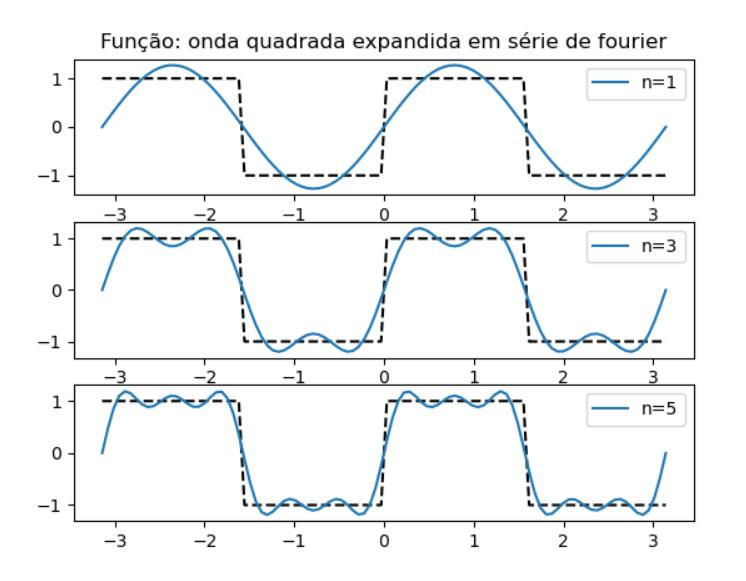
\includegraphics[scale=0.5]{fig1.png} % deve-se colocar o caminho da imagem entre as chaves
	\caption{Gráfico feito em Python} % legenda da imagem
	\label{grafico-python}
\end{figure}

Fazendo referência à imagem:

Podemo ver no gráfico da Figura \ref{grafico-python} que quanto maior o $n$ melhor a aproximação...

\end{document}